\section{Анализ дисцплин обслуживания ядра Linux}

    \subsection{Дисциплины обслуживания}

%    Добавить описание ДО. Рассказать про классовые и безклассовые.
%    Описать главные характеристики, которые будут в таблице.

	Дисциплина обслуживания очередей (ДО) -- правило выбора заявок
	из очереди для обслуживания\cite{Aliev}. В операционной системе Linux
	дисицплина обслуживания, обозначемая термином qdisc, используется
	для выбора пакетов из выходящей очереди для отправки на выходной интерфейс.
	Схема движения пакета приведена на Рисунке~\ref{pic:flow}. Выходная очередь
	обозначена термином egress; именно на этом этапе следования пакета
	и работает механизм qdisc.\cite{lartc}

    \begin{figure}[ht!]
        \center
        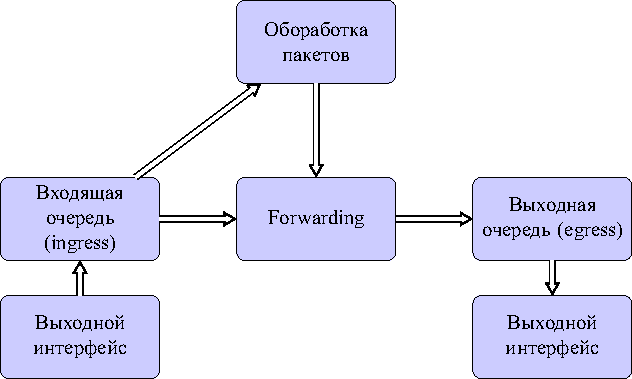
\includegraphics{pdfimages/qdisc.pdf}
        \caption{Схема движения пакета в системе Linux}
		\label{pic:flow}
    \end{figure}

	[Схема взята из TCP-IP Architecture. Как на это сослаться?]

	Возможно, нужно описать некоторые термины, которые потом будут представлены в таблице.

    \subsection{Приоритетные очереди}

    Приоритетные очереди (Priority Queueing, PQ) -- это техника обслуживания,
    при которой используется множество очередей с разными приоритетами. Очереди
    обслуживаются в циклическом порядке (алгоритмом round-robin) от самого высокого 
    до самого низкого приоритета; обслуживание следующей по порядку очереди происходит,
    если более приоритетные очереди пусты. Каждая очередь внутри обслуживается в порядке FIFO
    (First-In, First-Out). В случае переполнения отбрасываются пакеты из очереди
    с более низким приоритетом.\cite{packethandling}
    
    Дисциплина используется, чтобы понизить время отклика, когда нет нужды замедлять трафик. [mac tc-prio].

    В Linux алгоритм реализован в виде дисцплины prio, которая создаёт фиксированное
    значение очередей обслуживания, управляемые дисциплиной pfast\_fifo, и управляет
    очередями в соответствии с картой приоритетов.\cite{tcprio}

    \begin{figure}[ht!]
        \center
        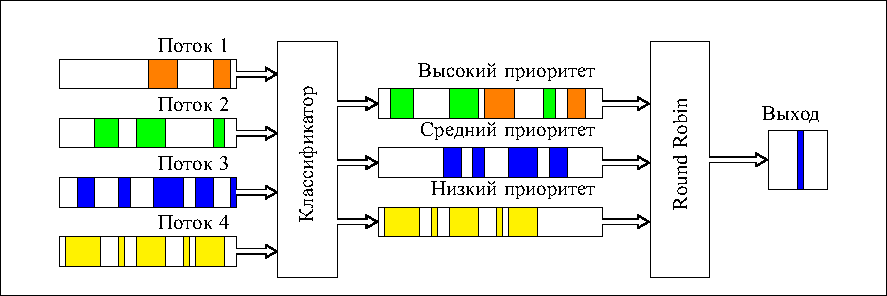
\includegraphics{pdfimages/pq.pdf}
        \caption{Схема обслуживания алгоритмом приоритетных очередей}
    \end{figure}

    Приемущества алгоритма состоят в следующем:
    \begin{itemize}
		\item возможность понижения времени отклика, когда нет необходимости замедлять трафик \cite{tcprio};
        \item наиболее простая в реализации классовая дисциплина обслуживания;
        \item для software-based маршрутизаторов PQ предоставляет относительно небольшую
             вычислительную нагрузку на систему в сравнении с более сложными ДО;
        \item PQ позволяет маршрутизаторам организовывать буферизацию пакетов и обслуживать
             один класс трафика отдельно от других. \cite{suppdiff}
    \end{itemize}

    Однако приоритетные очереди обладают рядом существенных недостатков.
    \begin{itemize}
        \item возникает проблема простоя канала (отсутствие обслуживания в течение продолжительного времени)
			  для низкоприоритетного трафика при избытке высокоприоритетного\cite{packethandling};
        \item избыточный высокоприоритетный трафик может значительно увеличивать
                задержку и джиттер для менее приоритетного трафика;
        \item не решается проблема с TCP и UDP, когда TCP-трафику даётся высокий приоритет и он
                пытается поглотить всю пропускную способность. \cite{suppdiff}
    \end{itemize}

    \subsection{Алгоритм управления очередями на основе классов}

        Алгоритм управления очередями на основе классов (Class Based Queueing, CBQ) -- это
        классовая дисциплина обслуживания, которая реализует
        иерархическое разделение канала между классами, и позволяет
        шейпинг трафика. \cite{tccbq}

        Главная цель CBQ -- это планировка пакетов в очередях, гарантия определённой
        скорости передачи и разделение канала. Если в очереди нет пакетов, её
        пропускная способность становится доступной для других очередей. Сила
        этого метода состоит в том, что он позволяет справляться со значительно
        различными требованиями к пропускной способности канала среди потоков. Это
        реализовано путём назначения определённого процента доступной ширины
        канала каждой очереди. CBQ избегает проблему простоя канала, которой страдает
        алгоритм PQ, так как как минимум один пакет обслуживается от каждой очереди
        в течение цикла обслуживания.\cite{packethandling}

		Алгоритм CBQ представляет канал в кажется иерархической структуры \cite{linksharing},
		пример которой представлен на Рисунке~\ref{cbq}. Голубым цветом обозначен узел,
		представляющий собой основной канал; он разделяется между двумя классами трафика:
		интеркативным (левый узел) и остальным (правый узел), -- которым назначается процент
		пропускной способности от остального канала. Весь трафик, причиляемый к классу,
		будет получать выделенную пропускную способность для этого класса. Эти
		классы трафика могут разделяться на подклассы и так далее. Если класс не использует
		пропускную способность, она будет выделяться классу-соседу. Этот механизм
		называется механизмом разделения канала \cite{linksharing}. 

        \begin{figure}[ht!]
			\center
            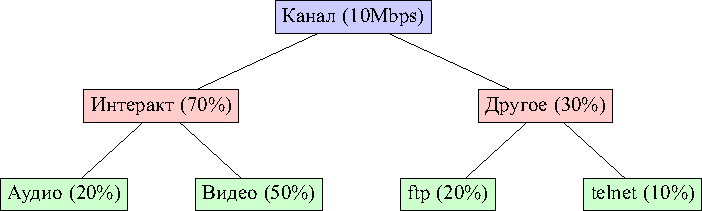
\includegraphics[scale=1.2]{./pdfimages/cbq.pdf}
            \caption{Разделение канала при CBQ}
			\label{cbq}
        \end{figure}

        Алгоритм CBQ состоит в следующем. Сначала пакеты классифицируются в классы
        обслуживания в соответствии с определёнными критериями и сохраняются в
        соответствующей очереди. Очереди обслуживаются циклически. Различное
        количество пропускной способности может быть назначено для каждой очереди
        двумя различными способами: с помощью позволения очереди отправлять более
        чем один пакет на каждый цикл обслуживания или с помощью позволения очереди
        отправлять только один пакет за цикл, но при этом очередь может быть обслужена
        несколько раз за цикл.\cite{packethandling}

        Преимущества алгоритма состоят в следующем:
        \begin{itemize}
            \item позволяет контролировать количество пропускной способности для каждого
                  класса обслуживания;
            \item каждый класс получает обслуживание, вне зависимости от других классов. Это
                  помогает избегать проблемы PQ, когда при избытке высокоприоритезированного
                  трафика низкоприоритезированный не обслуживался вообще.\cite{packethandling}
        \end{itemize}

        Недостатки же в большей следуют из особенностей реализации алгоритма в системе Linux:
        \begin{itemize}
            \item честное выделение пропускной способности происходит, только если
                  пакеты из всех очередей имеют сравнительно одинаковый размер. Если один класс
                  обслуживания содержит пакет, который длиннее остальных, этот класс обслуживания
                  получит большую пропускную способность, чем сконфигурированное значение \cite{packethandling};

            \item высокая сложность реализации. В ядре Linux реализация СBQ приближённая и
                  в некоторых случаях может давать неверные результаты. (в комментариях к коду)
        \end{itemize}
        %(Более полное описание есть в man tc-cbq, ругают в http://tldp.org/HOWTO/Adv-Routing-HOWTO/lartc.qdisc.classful.html
        %судя по http://web.opalsoft.net/qos/default.php?p=ds-28).

    \subsection{Алгоритм иерархического маркерного ведра}

        Алгоритм иерархического маркерного ведра (Hierarchical Token Bucket, HTB) -- дисциплина
        обслуживания с иерархическим разделением канала между классами.

	


		HTB состоит из произвольного числа иерархически организованных фильтров маркерного
        ведра (Token Bucket Filter, TBF). \cite{packethandling}

		HTB, подобно CBQ, использует механизм разделения канала. 

		HTB позволяет создать динамическую структуру разделения
		канала основанного на дереве, где узел определяет класс,
		а его потомки -- некоторый подкласс; каждому классу
		выделяется пропускная способность, которая разделяется
		между подклассами.

% Это можно опистать короче.
%		 HTB ensures that the amount of service provided to each class is at least the minimum of the amount it
%		 requests and the amount assigned to it. When a class requests less than the amount assigned, the remaining
%		 (excess) bandwidth is distributed to other classes which request service.
%
%		HTB обеспечивает, что количество обслуживания, предоставляемое каждому классу, является,
%		минимальным значением из запрошенного количество и назначенного классу. Когда класс
%		запрашивает меньше, чем ему выделенно, оставшаяся пропускная способность распределяется между
%		другими классами, которое требует ..


%		
%		Если подкласс не использует назначенную пропускную способность, она распределяется между
%        его соседями; если на более высоком уровне иерархии класс не использует
%        всю пропускную способность, она распределяется уже между соседями этого
%        класса. Сами очереди содержатся в листьях дерева.
%
%        Алгоритм похож на Class-Based Queueing, и по сути является ещё одной реализации
%        формального похода разделения канала.
%
%        При добавлении пакета в очередь HTB начинает обход дерева от корня
%        для определения подходящей очереди: в каждом узле происходит поиск
%        инструкций, и затем происходит переход в узел, на который ссылается
%        инструкция. Обход заканчивается, когда алгоритм доходит до листа,
%        в очередь которого помещается пакет. 

        \begin{figure}[ht!]
            \center
            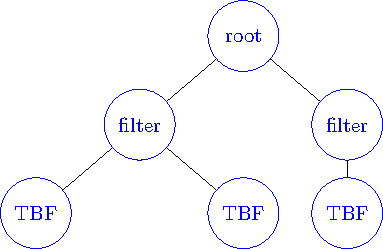
\includegraphics{./pdfimages/class_hierh_htb.pdf}
            \caption{Пример иерархии классов при использовании дисицплины HTB}
        \end{figure}


        Приемущества.
        \begin{itemize}
            \item Наиболее используется дисциплина обслуживания в Linux.
            \item Иерархическая структура предоставляет гибкую возможность конфигурировать трафик.
            \item Не зависит от характеристик интерфейса и не нуждается в знании о лежащей в
                  основе пропускной способности выходного интерфейса из-за свойств TBF. [man tc-htb]
            \item Вычислительно проще, чем алгоритм CBQ.
        \end{itemize}

        Недостатки.
        \begin{itemize}
            \item Медленее CBQ в N раз, где N -- глубина дерева разделения, что, однако, компенсируется простотой вычислений. 
            \item Видимо, связаны с TBF.
        \end{itemize}

    \subsection{Алгоритм иерархических честных кривых обслуживания}
% https://www.cs.cmu.edu/~hzhang/papers/SIGCOM97.pdf
% http://linux-tc-notes.sourceforge.net/tc/doc/sch_hfsc.txt
% https://serverfault.com/questions/105014/does-anyone-really-understand-how-hfsc-scheduling-in-linux-bsd-works

        HFSC -- Hierarchical Fair-Service Curve -- иерархический алгоритм планирования пакетов,
        основанный на математической модели честных кривых обслуживания (Fair Service Curve),
        где под термином “кривая обслуживания” подразумевается зависящая от времени
        неубывающая функция, которая служит нижней границей количества обслуживания,
        предоставляемого системой [из сетевого исчисления, ссылка на какой-либо ресурс
        такого рода].

    
        HFSC ставит перед собой цели:
        \begin{itemize}
            \item гарантировать точное выделение пропускной способности и задержки для всех листовых классов (критерий реального времени);
            \item честно выделять избыточную пропускную способность как указано классовой иерархией (критерий разделения канала);
            \item минимизировать несоответствие кривой обслуживания идеальной модели и действительного количество обслуживания. [man 7 tc-hfsc]
        \end{itemize}

        Алгоритм планировки основан на двух критериях: критерий реального времени
        (real-time) и критерий разделения канала (link-sharing). Критерии реального времени
        используются для выбора пакета в условиях, когда есть потенциальная опасность,
        что гарантия обслуживания для листового класса нарушается. В ином случае
        используется критерий разделения канала.

        HFSC использует три типа временных параметров: время крайнего срока (deadline
        time), <<подходящее>> время (eligible time) и виртуальное время (virtual time). Время крайнего
        срока назначается таким образом, чтобы, если крайние сроки всех пакетов сессии
        выполнены, его кривая была гарантирована. <<Подходящее>> время используется для
        выбора критерия планировки для следующего пакета. Виртуальное время показывает
        нормализованное количество обслуживания, которое получил класс. Виртуальное
        время присуще всем вершинам дерева классов, так как является важным параметром
        при критерии разделение канала, при котором должно минимизироваться
        несоответствие между виртуальным временем класса и временами его соседей
        (так как в идеальной модели виртуальное время соседей одинаково); при выборе
        критерия разделения канала алгоритм рекурсивно, начиная с корня, обходит всё
        дерево, переходя в вершины с наименьшим виртуальным временем. Время крайнего
        срока и <<подходящее>> время используются дополнительно в листьевых классах,
        так как в этих вершинах непосредственно содержатся очереди. [SIGCOM97.pdf, описать
        более вразумительно].

        Преимущества.
        \begin{itemize}
            \item Алгоритм основан на формальной модели с доказанными нижними границами.
        \end{itemize}

        Недостатки.
        \begin{itemize}
            \item Сложность.
        \end{itemize}

    \subsection{Flow-based WFQ}

    WFQ (Weighted Fait Queueing) -- динамический метод планировки пакетов, который
    предоставляет честное разделение пропускной способности всем потокам трафика.
    WFQ применяет вес, чтобы идентифицировать и классифицировать трафик
    в поток и определить, как много выделить пропускной способности каждому
    потоку относительно других потоков. WFQ на месте планирует интерактивный трафик в начало очереди,
    уменьшая там самым время ответа, и честно делит оставшуюся пропускную
    способность между остальными потоками. 
    [link]
    % https://www.cisco.com/c/en/us/td/docs/ios/12_2/qos/configuration/guide/fqos_c/qcfconmg.html

    [Картинка]
    
    \begin{figure}[ht!]
			\center
        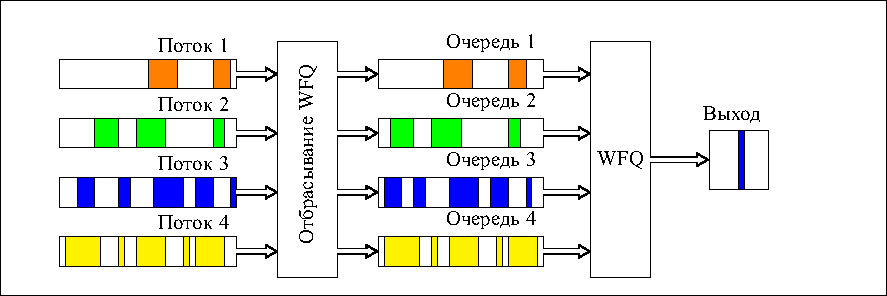
\includegraphics{./pdfimages/fwfq.pdf}
        \caption{Схема WFQ системы}
    \end{figure}

    %В соответствии с механизмом WFQ вес пакета определяется на основании значения поля
    %IP-приоритета в заголовке пакета $\text{вес} = 4096 \div (\text{IP-приоритет} + 1)$
    %(в новых версиях $32768 \div (\text{IP-приоритет} + 1)$). 
    %Вес пакета строго зависит от его приоритета и не может
    %быть изменён.

    Планировщик не нарушает порядка обработки пакетов,
    принадлежащих одному потока, даже в том случае, если они имеют различный приоритет.
    C этой целью поток реализуется в виде хэша, определяемого IP-адресом источника,
    IP-адресом цели назначения, полем протокола IP, номерами портов TCP/UDP и пятью
    битами байта ToS (Type of Service).Очередь потока обслуживается в соответствии с алгоритмом FIFO.

    % Алгоритм WFQ отбрасывает пакеты только наиболее активных потоков трафика.

    WFQ на основе потока использует для обработки каждого трафика так называемые
    очереди диалога (conversation queue).
    Поскольку память -- конечный ресурс, число очередей диалога по умолчанию
    ограничено 256. Если число потоков превысит число очередей, допускается
    использование одной очереди для обработки нескольких потоков.[вегешн]

    В целях планировки в WFQ длина очереди измеряется не в пакетах, а во времени,
    которое заняла бы передача всех пакетов в очереди. WFQ адаптирует количество
    потоков и выделяет одинаковое количество полосы пропускания каждому потоку.
    Поток с маленькими пакетами, которые обычно являются интерактивными потоками,
    получают лучшее обслуживание, потому что они не нуждаются в большой полосе пропускания;
    также они получаются низкую задрежку, потому что у меньших пакетов меньшее
    время отправки (finish time). Время отправки -- это сумма текущего времени и
    время, которое заняла бы отправка пакета. Текущее время ноль, если в очереди
    нет пакетов. WFQ поместит пакет в аппаратную очередь, основываясь на времени отправки в
    порядке возрастания.

    Чтобы ввести вес в расчёт то, в каком порядке будут обслуживаться очереди,
    WFQ использует время окончания и приоритет IP (IP precedence). Вес расчитывается
    как время окончания, делённое на приоритет IP плюс один (во избежание деления
    на ноль). Однако для увеличения производительности в маршрутизаторах Cisco
    взамен времени отправки (finish time) используется размер пакета, так как он
    пропорционален времени; к тому же деление на приоритет IP заменяется на умножение
    фиксированного значения, просчитанного заранее (это сделано из-за того,
    что деление более трудная операция для CPU, чем умножение).

    WFQ использует два метода отбрасывания пакетов: ранее (Early Dropping) и агрессивное
    (Aggressive Dropping) отбрасывания. Ранее отбрасывание срабатывает тогда, когда
    достигается congestive discard threshold (CDT); CDT -- это количество пакетов, которые могут
    находиться в системе WFQ перед тем, как начнётся отбрасывание новых пакетов
    из самой длиной очереди; используется, чтобы начать отбрасывание пакетов
    из наиболее агрессивного потока, даже перед тем, как достигнется предел
    hold queue out (HQO). HQO -- это максимальное количество пакетов, которое может быть
    во всех выходящих очередях в интерфейсе в любое время; при достижении HQO
    срабатывает агрессивный режим отбрасывания.

    \begin{figure}[ht!]
			\center
        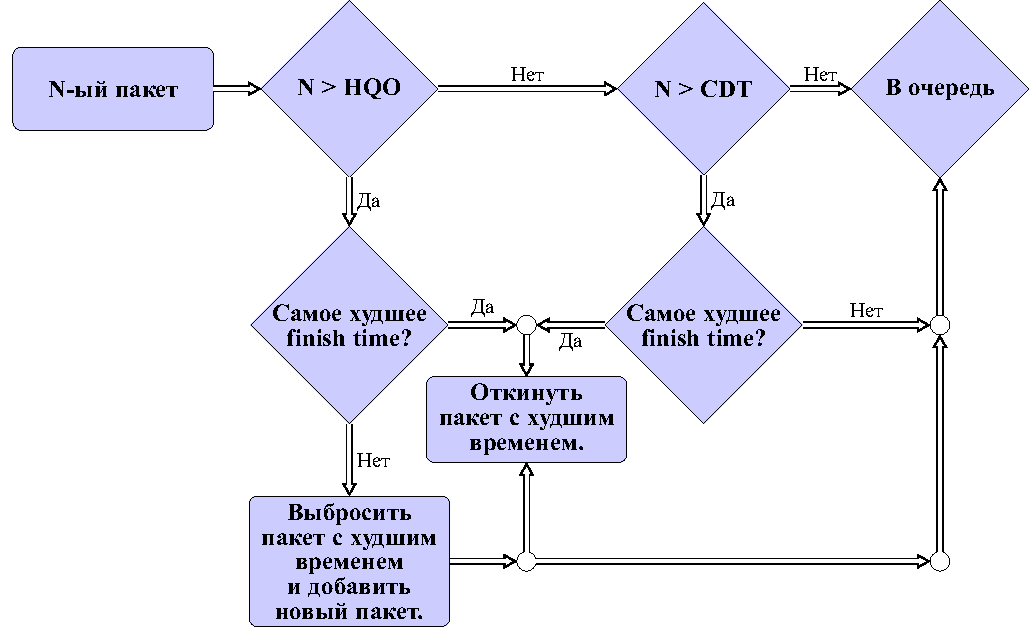
\includegraphics{./pdfimages/fwfq_drop.pdf}
        \caption{Схема отбрасывания пакетов WFQ}
    \end{figure}
    [\url{http://blog.globalknowledge.com/2010/02/12/quality-of-service-part-10-weighted-fair-queuing/}]

    % В WFQ (см. рис. "WFQ-drop.png"):
    % 1. При поступлении нового пакета в WFQ система сравнивает число пакетов во
    %    всех очередях с hold-queue limit (заданный макс. размер всех WFQ очередей).
    % 2. Если этот лимит перевышен, то определяется пакет с самым большим временем на передачу (Worst Finish Time*), это может быть как новый пакет, так и уже содержащийся в одной из очередей.
    % 3. Пакет с самым большим Worst Finish Time отбрасывается (если это не новый пакет, то он передается в очередь).
    % 4. Если hold-queue limit не превышен, то пакет попадает в очередь, затем длина этой очереди сравнивается с congestive-discard-threshold - макс. размер очереди.
    % 5. Если congestive-discard-threshold не превышен, то пакет обрабатывается дальше.
    % 6. Если congestive-discard-threshold превышен, то анализируется его Worst Finish Time, если оно самое большое , то он отбрасывается, в противном случае пакет обрабатывается дальше.
    % 7. Пакет, который направляется в пустую очередь, не отбрасывается.
    % Worst Finish Time* = время обработки в очереди предыдущего пакета + время на передачу (обработку) пакета
     
    Приемущества.
    \begin{itemize}
        \item Простая конфигурация.
        \item Гарантированная полоса пропускания для всех потоков.
        \item Отбрасывание пакетов из более агрессивных потоков.
    \end{itemize}

    WFQ страдает от нескольких недостатков.
    \begin{itemize}
        \item  Трафик не может регулироваться на основе пользовательски определённых классов.
        \item  WFQ не может предоставить фиксированную пропускную способность.
        \item  WFQ поддерживается только на медленных каналах.
    \end{itemize}
    % http://www.routeralley.com/guides/qos_queuing.pdf

    Эти ограничения были исправлены CBWFQ.

    \subsection{Class-Based WFQ}

    % https://www.cisco.com/en/US/docs/ios/12_0t/12_0t5/feature/guide/cbwfq.html
%   Надо описать, что было создано в Cisco и т.п. и как это работает в циско.
%   Таблица сравнений с flow-based WFQ
%   Предоставляет одну очередь для класса, всего 64 класса.
%   Позволяет указывать пропускную способность для класса
%   Предоставляет гарантию пропускной способности для пользовательких классов.
%   Предоставляет поддержку flow-based WFQ для не определёнными пользователями
%   трафиков класса.
%   Требует конфигурацию.
%   [cм ссылку в комментах]
    % https://www.cisco.com/c/en/us/td/docs/ios/12_2/qos/configuration/guide/fqos_c/qcfconmg.html

    CBWFQ (Class-based weighted fair queueing) -- основанный на классах взвешенный алгоритм равномерного обслуживания 
    очередей[вагешен?]; является расширением функциональности дисциплины обслуживания WFQ,
    основанной на потоках, для предоставления определяемых пользователями классов трафика. 

    Сlass-Based WFQ -- это мехнизм, использующийся для гарантировании пропускной способности
    для класса. Для CBWFQ класс трафика определяется на основе заданных криетриев
    соответствия: список контроля доступа (ACL), протокол, входящий интерфейс и т.п. Пакеты,
    удовлетворяющие криетриям класса, составляют трафика для этого класса. Дисциплина
    позволяет задавать до 64-х пользовательских классов.

    После определения класса, ему назначаются характеристики, которые определяют
    политику очереди: пропускная способность, выделенная классу, максимальная
    длина очереди и так далее.[link] Алгоритм CBWFQ позволяет явано указать требуемую минимальную
    полосу пропускания для каждого класса трафика.[вегешн] Полоса пропускания используется
    в качестве веса класса. Вес можно задать в абсолютной (опция \texttt{bandwidth}),
    в процентной (опция \texttt{bandwidth percent}) и в доле от оставшиейся
    полосы пропускания (опция \texttt{bandwidth remaining precent}) величинах.

    Кроме пользовательских классов CBWFQ предоставляет стандартный класс (default class),
    в который попадает весь трафик, который не был классифицирован. В стандартном классе
    управление очередью может осуществляться с помощью алгоритмов FIFO и FQ (Fair Queueing). 

    В случае переполнения очередей начинает работать алгоритм отбрасывания пакетов.
    В качестве политики отбрасывания пакетов по умолчанию используется отбрасывание конца
    очереди (Tail Drop), однако допускается сконфигуривать работу
    алгоритм взвешенного произвольного раннего обнаружения (Weighted Random Early Detection, WRED)
    для каждого класса.

    
    [вставить картинку]

    Больше Cisco-реализации.

    % [link]

    %Для CBWFQ класс трафика определяется
    %на основе критериев соответствия, которые могут включать в себя протокол,
    %список контроля доступа (ACL) и входящий интерфейс. Пакеты, удовлетворяющие
    %критериям для класса, составляют трафик для этого класса. После определения
    %класса критериями соответствия, ему назначаются характеристики: пропускная
    %способность, вес, максимальная длина очереди и максимальное количество
    %пакетов. Пропускная способность, которая назначается классу, является
    %гарантированной и предоставляется классу в течение перегрузки.

